\chapter{Language Modeling}
\label{chap:language-modeling}
This chapter presents the results of this thesis. The chapter starts with ... the research questions defined in \cref{sec:research-questions}.

As discussed in section \cref{sec:transformers-for-code-synthesis}, there are several available transformer models. However, only a few of them have open-sourced pre-trained weights. Of these, only GPT-J \cite{gpt-j} includes code in it's pre-training dataset "The Pile", described in \cref{sec:the-pile}. As GPT-J is a state-of-the-art generative pre-trained transformer model, this is the language model used in this thesis. This chapter presents a detailed overview of the system architecture for generating secure Smart Contract code. The first section gives an overview of the GPT-J model architecture, followed by a section describing the pre-training of the model. The third section describes the fine-tuning process on the smart contract dataset presented in \cref{sec:verified-smart-contracts-inflated,sec:verified-smart-contracts-audit}. 

\todo{Add figure of training process}

\section{Model architecture}
\label{sec:architecture}
Ever since OpenAI introduced its first transformer model in the GPT series, this class of transformers has been touted as the state-of-the-art for text generation. Their latest model, GPT-3 \cite{brown2020language}, is their best performing model with 175 billion parameters. However, the model is not openly available at the current time. GPT-J \cite{gpt-j} with 6 billion parameters (GPT-J-6B) is currently one of the best open-source alternatives to OpenAI's GPT-3. GPT-J was released in June 2021 by EleutherAI \cite{elutherai}, a grassroots collection of researchers working to open-source AI research. The model is trained on the Pile, an 825 GiB diverse, open-source language modeling data set that consists of 22 smaller, high-quality datasets combined together. See section \cref{sec:the-pile} for a more detailed description of the Pile.

Being a GPT class transformer, GPT-J uses a decoder-only architecture, as can be seen in \cref{fig:gpt-j-architecture}. The GPT-J introduces some notable differences from standard transformer models. Firstly, instead of computing attention and feed-forward layers in sequential order, they are computed in parallel and the results are added together. This decreases communication during distributed training, resulting in increased throughput. Secondly, GPT-J uses \acrfull{rope} \cite{su2021roformer} for position encoding. Opposite to sinusoidal encoding used in standard transformer models (see \cref{sec:embedding-and-positional-encoding}), this is shown to result in better model quality in tasks with long text \cite{su2021roformer}.

\begin{figure}[htp]
    \centering
    %\def\svgwidth{\linewidth}
    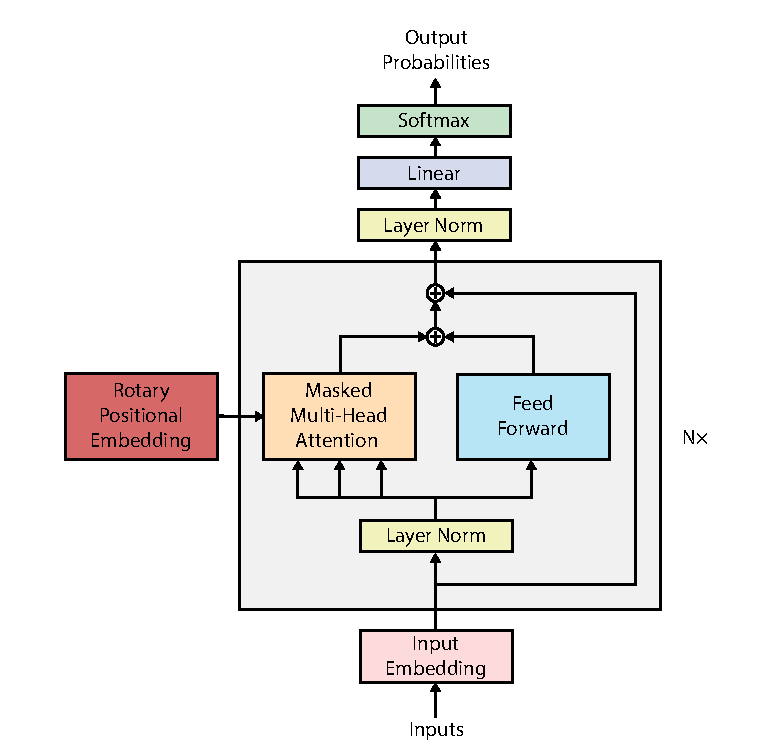
\includegraphics[width=0.8\textwidth]{figures/gpt-j_architecture.pdf}
    \caption{Diagram of GPT-J model architecture}
    \label{fig:gpt-j-architecture}
\end{figure}

\section{Requirements}
\label{sec:requirements}
To load the GPT-J model in float32 precision, one would need at least 2x the model size of CPU RAM: 1x for the initial weights and another 1x to load the checkpoint. So for just loading the GPT-J model, it would require at least 48GB or CPU RAM. To reduce the memory footprint, one can load the model in half-precision.

GPU needs around 40GB of GPU memory to load the model. For training/fine-tuning the model, it would require significantly more GPU RAM. For example, the Adam optimizer makes four copies of the model: model, gradients, average and the squared average of gradients. Hence, it would take 4x model size GPU memory, even with mixed precision as gradient updates are in fp32. Further, this doesn't include the activations and data batches which would require some more GPU RAM. Hence, solutions like DeepSpeed needs to be used for training/fine-tuning such large models.

If a GPU with mixed precision capabilities (architecture Pascal or more recent) is available, one can use mixed precision training with PyTorch 1.6.0 or later, or by installing the Apex library for previous versions. If using an NVIDIA “Ampere” GPU architecture, the Brain Floting Point (BF16) floating-point format can be used. Using mixed precision training usually results in 2x-speedup for training with the same final results.

\section{Pre-training}
\label{sec:pretraining}
Pre-training is defined as "Training in advanced". By first training the model on a huge dataset, the model can then be fine-tuned on a much smaller dataset. This is so-called transfer learning. In this project, pre-trained weights for GPT-J-6B from ElutherAI are used. The pre-training by ElutherAI is done on the dataset The Pile, described in \cref{sec:the-pile}. Of the roughly 825GiB, 95.16 GiB (7.59\%) of The Pile is code from GitHub. Compared to many other open-source models, GPT-J-6B is one of the most promising models for the task of code generation.

The specific GPT-J model configuration can be seen in \cref{tab:gpt-j-model-details}. In detail, GPT-J-6B consists of 28 layers with a model dimension of 4096, and a feedforward dimension of 16384. The model dimension is split into 16 heads, each with a dimension of 256. \acrfull{rope} is applied to 64 dimensions of each head. The model is trained with a tokenization vocabulary of 50257, using the same set of \acrfullpl{bpe} as GPT-2 and GPT-3. The weights of GPT-J-6B are licensed under version 2.0 of the Apache License.


%Total params: 6,050,882,784
%multi-layer perceptron (MLP)

\begin{table}
    %\newcolumntype{Y}{>{\centering\arraybackslash}X}
    \def\arraystretch{1.5}
    \small
    \centering
    \caption{GPT-J-6B model details.}
    \label{tab:gpt-j-model-details}
    \begin{tabularx}{\textwidth}{XX}
        \toprule
        \textbf{Hyper parameter} & \textbf{Value}\\
        \midrule
        n\_parameters & 6,053,381,344\\
        n\_layers & 28*\\
        d\_model & 4,096\\
        d\_ff & 16,384\\
        n\_heads & 16\\
        d\_head & 256\\
        n\_ctx & 2,048\\
        n\_vocab & 50,257 (same tokenizer as GPT-2/3)\\
        position \& encoding & \acrfullpl{rope}\\
        RoPE dimensions & 64\\
        \bottomrule
    \end{tabularx}
\end{table}

\todo{add table notes}
* each layer consists of one feedforward block and one self attention block


\section{Fine-tuning}
\label{sec:fine-tuning}
To improve the pre-trained GPT-J-6B model's smart contract code generation performance, the model is fine-tuned on a dataset only containing real Ethereum Smart Contract code. Specifically, two models are created. The first model, named GPT-J-6B-Smart-Contract, is fine-tuned on the Verified Smart Contracts dataset \cref{sec:verified-smart-contracts}. The other model, named GPT-J-6B-Smart-Contract-Audit, is a secure version of the first model. It is fine-tuned on the Verified Smart Contracts Audit dataset \cref{sec:verified-smart-contracts-audit}, the same dataset as for the first model but with additional labeling from vulnerability analysis.

\begin{table}
    %\newcolumntype{Y}{>{\centering\arraybackslash}X}
    \def\arraystretch{1.5}
    \small
    \centering
    \caption{Hyper parameters for GPT-J model}
    \label{tab:inclusion-exclusion-criteria}
    \begin{tabularx}{\textwidth}{XX}
        \toprule
        \textbf{Hyper parameter} & \\
        \midrule
        \_name\_or\_path & EleutherAI/gpt-j-6B\\
        activation\_function & gelu\_new\\
        architectures & GPTJForCausalLM\\
        attn\_pdrop & 0.0\\
        bos\_token\_id & 50256\\
        embd\_pdrop & 0.0\\
        eos\_token\_id & 50256\\
        gradient\_checkpointing & false\\
        initializer\_range & 0.02\\
        layer\_norm\_epsilon & 1e-05\\
        model\_type & gptj\\
        n\_embd & 4096\\
        n\_head & 16\\
        n\_inner & null\\
        n\_layer & 28\\
        n\_positions & 2048\\
        resid\_pdrop & 0.0\\
        rotary & true\\
        rotary\_dim & 64\\
        scale\_attn\_weights & true\\
        summary\_activation & null\\
        summary\_first\_dropout & 0.1\\
        summary\_proj\_to\_labels & true\\
        summary\_type & cls\_index\\
        summary\_use\_proj & true\\
        tie\_word\_embeddings & false\\
        tokenizer\_class & "GPT2Tokenizer"\\
        transformers\_version & "4.19.0.dev0"\\
        use\_cache & true\\
        vocab\_size & 50400\\
        \bottomrule
    \end{tabularx}
\end{table}


\begin{table}
    %\newcolumntype{Y}{>{\centering\arraybackslash}X}
    \def\arraystretch{1.5}
    \small
    \centering
    \caption{DeepSpeed Zero config.}
    \label{tab:inclusion-exclusion-criteria}
    \begin{tabularx}{\textwidth}{XX}
        \toprule
        \textbf{Hyper parameter} & \\
        \midrule
        stage & 2\\
        contiguous\_gradients & true\\
        reduce\_scatter & true\\
        reduce\_bucket\_size & 2.000000e+08\\
        allgather\_partitions & true\\
        allgather\_bucket\_size & 2.000000e+08\\
        overlap\_comm & true\\
        load\_from\_fp32\_weights & true\\
        elastic\_checkpoint & false\\
        offload\_param & null\\
        \midrule
        offload\_optimizer & device: null\\
        & nvme\_path: null\\
        & buffer\_count: 4\\
        & pin\_memory: false\\
        & pipeline\_read: false\\
        & pipeline\_write: false\\
        & fast\_init: false\\
        \midrule
        sub\_group\_size & 1.000000e+09\\
        prefetch\_bucket\_size & 5.000000e+07\\
        param\_persistence\_threshold & 1.000000e+05\\
        max\_live\_parameters & 1.000000e+09\\
        max\_reuse\_distance & 1.000000e+09\\
        gather\_16bit\_weights\_on\_model\_save & false\\
        ignore\_unused\_parameters & true\\
        round\_robin\_gradients & false\\
        legacy\_stage1 & false\\
        \bottomrule
    \end{tabularx}
\end{table}

\section{Inference}

TODO: What is supported by the model? How much memory to use?
We perform beam search with width of 5 and optimize for accuracy@1


\section{Security Conditioning}
\label{sec:security-conditioning}
When training a large language model on several gigabytes of open-source code, it is safe to assume that large portions of this code are not safe and contains vulnerabilities. In the case of Smart Contracts, the vulnerability analysis presented in section \ref{sec:verified-smart-contracts} shows that almost 50\% of deployed Smart Contracts contain at least one high-severity vulnerability. This will result in a biased model that may produce a lot of vulnerable code. This section introduces a technique, named security conditioning, to reduce and mitigate this problem.

Vulnerability analysis is a difficult area. It is especially hard in the area of smart contracts, where the execution environment is not deterministic ????\todo{find correct wording.}... Previous works have tried to classify vulnerable code with large language models without much success \todo{Cite previous works}. In this project, instead of classifying vulnerable code, the goal is to make the model more secure by conditioning it on the presence of vulnerabilities.

The security conditioning is done by appending a special security label to each of the records in the training data. This way, the model can use this token(s) to condition whether to produce safe or vulnerable code. This requires the dataset to first be labeled as secure or vulnerable. For this project, SolidityDetector is used for labeling. Further details on the dataset construction can be found in \cref{sec:verified-smart-contracts-audit}.

\todo{Add example of security conditioning.}